\chapter{Software}
\label{cha:software}

Wie bereits in Kapitel \ref{cha:Einleitung} erwähnt, war die Nachimplementierung/Simulation von Spe\_ed unser erster Implementierungsschritt. Da die eingesetzten Modellierungstechniken- und Frameworks einen maßgeblichen Einfluss auf die gesamte Architektur haben, stellen wir unser Vorgehen bei der Modellierung in diesem Kapitel genauer vor. Außerdem gehen wir auf die Punkte Software-Architektur, Software-Testing und Wartbarkeit/Erweiterbarkeit ein.

Zunächst noch ein paar allgemeinere Angaben zur Software: Wir haben uns für die Programmiersprache \textit{Python} entschieden, da sie ein breites Spektrum an bewährten Werkzeugen für Modellierung, \acrshort{RL} und Datenanalyse bietet. Wir verwenden die Python-Version 3.7, unsere Implementierungen sind streng nach den Coding Conventions des \textit{PEP 8 Style Guide}\footnote{https://www.python.org/dev/peps/pep-0008/} formatiert und \textit{Core}-Klassen und -Funktionen sind durchgehend mit \textit{Docstrings}\footnote{https://www.python.org/dev/peps/pep-0257/} dokumentiert.

\section{Architektur und Modellierung}
\label{sec:modellierung}

Die Software-Architektur unseres Projektes ist in die Software-Pakete \textit{Core}, \textit{Evaluation} und \textit{Scripts} geteilt. \textit{Core} stellt den funktionalen Kern unseres Projekts dar. Es enthält das Spe\_ed-Modell und die implementierten Spieler-Algorithmen (\textit{Agents}). \textit{Evaluation} beinhaltet unsere Auswertungssoftware und \textit{Scripts} enthält beispielsweise Skripte zur Online-Ausführung unserer Agenten. Abbildung \ref{fig:komponentendiagramm} zeigt den beschriebenen Aufbau und die Abhänigkeitshirarchie zwischen den Software-Paketen.

\begin{figure}[ht]
    \centering
    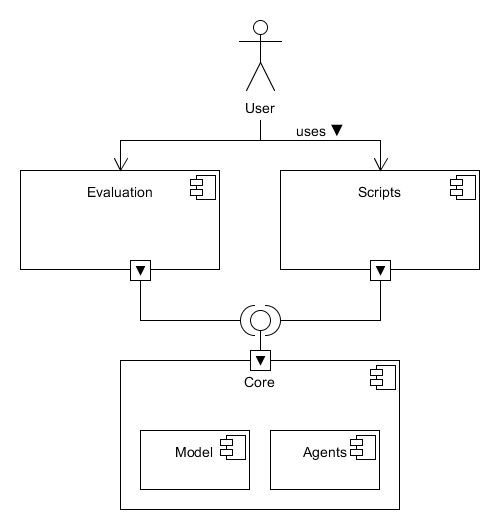
\includegraphics[width=0.7\textwidth]{img/architecture.png}
    \caption{Komponentendiagramm unseres Projekts}
	\label{fig:komponentendiagramm}
\end{figure}

Unsere grundlegende Idee hinter der Modellierung von Spe\_ed ist, dass das Modell wie eine Black-Box verwendet werden kann, deren Schnittstellen mit denen des originalen Spiels übereinstimmen. Die Input- und Output-Formate des Modells entsprechen daher exakt den JSON-Formaten des originalen Spiels. Somit kann eine entwickelte Spieler-Software ohne Änderungen sowohl im Modell als auch im Original ausgeführt werden.

Als Modellierungsansatz haben wir uns für \acrfull{ABM} entschieden. \acrshort{ABM} verfolgt einen \textit{Bottom-Up}-Ansatz zur Modellierung von Simulationen. Das bedeutet, dass der Ablauf der Simulation nicht zentral von ’oben’ herab gesteuert wird, sondern dass die autonomen Individuen der Simulation (genannt \textit{Agenten}) den Simulationsverlauf durch ihr jeweiliges Verhalten von ’unten’ aus bestimmen. Die zentralen Komponenten von \acrshort{ABM} sind (1) mehrere Agenten und (2) die Umgebung, in der sich die Agenten befinden. \acrshort{ABM} eignet sich besonders gut zur Modellierung und Simulation von Spe\_ed, da Spe\_ed ein Multi-Agenten-System ist, in dem die Agenten ein eigenes - nicht zentral vorgegebenes - Verhalten besitzen. Bei Simulationen wird zudem zwischen \textit{ereignisbasierten} (auch \textit{asynchronen}) und \textit{zeitorientierten} (auch \textit{synchronen}) Modellen unterschieden. Bei Spe\_ed handelt es sich um ein System in dem alle Agenten in festen Zeitschritten eine Entscheidung treffen. Deshalb ist es sinnvoll ein zeitorientiertes Modell zu wählen. \cite{Bernhardt.2007, Macal.2009}

Um unsere Software möglichst effizient, wartbar und leicht verständlich zu gestalten nutzen wir ein Simulationsframework. Auf Basis der oben genannten Kriterien haben wir \textit{Mesa} \cite{Masad.2015} als Framework für die Implementierung unseres Spe\_ed-Modells gewählt. Mesa wurde 2015 als erstes \acrshort{ABM}-Framework für Python veröffentlicht. Es ist \textit{open-source} und orientiert sich an anderen \acrshort{ABM}-Tools und -Frameworks, wie \textit{NetLogo} \cite{Wilensky.2004}, \textit{Repast} \cite{North.2013} und \textit{MASON} \cite{Luke.2005}. Mesa besitzt zudem einen leichtgewichtigen und somit effizienten Framework-Kern. Das Framework ordnet seine Komponenten drei verschiedenen Modulen zu: Modellierung, Visualisierung und Analyse. Wir beschäftigen uns im Folgenden zwar lediglich mit der Modellierung, allerdings ist es nennenswert, dass wir unser Modell durch die Nutzung von Mesa ohne beachtlichen Mehraufwand web-basiert visualisieren und analysieren können.

Das Modellierungsmodul von Mesa implementiert den \acrshort{ABM}-Ansatz. Es besteht aus den Basisklassen \textit{Model}, \textit{Agent}, \textit{Scheduler} und \textit{Space}. Die \textit{Model}-Klasse enthält Modellparameter und steuert (startet, stoppt, etc.) den Ablauf einer Simulation. In der \textit{Agent}-Klasse wird definiert, welche Prozesse ein Agent bei seiner Aktivierung durchläuft - die Aktivierung eines Agenten entspricht bei uns der Ausführung eines Zuges. Der \textit{Scheduler} verwaltet die Simulationszeit. Er kennt alle Agenten und aktiviert diese in jedem Zeitschritt. Die \textit{Space}-Klasse beschreibt den Raum, in dem sich die Agenten befinden. Mesa bietet von Haus aus mehrere Unterklassen der \textit{Scheduler}- und \textit{Space}-Klassen an. In unserem Anwendungsfall wird der \textit{SimultaneousActivation}-Scheduler und der \textit{MultiGrid}-Space verwendet.

\begin{figure}[ht]
    \centering
    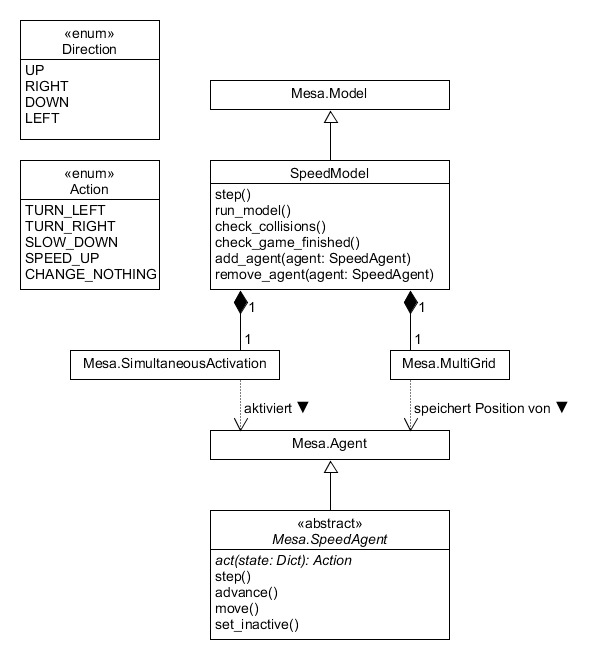
\includegraphics[width=0.8\textwidth]{img/model.png}
    \caption{Vereinfachtes Klassendiagramm der Modell-Architektur}
	\label{fig:model}
\end{figure}

Abbildung \ref{fig:model} zeigt ein vereinfachtes Klassendiagramm unserer Modell-Architektur. Klassen die Bestandteil von Mesa sind, sind mit dem Präfix \textit{Mesa.} versehen. Im Mittelpunkt stehen die Klassen \textit{SpeedModel} und \textit{SpeedAgent}. Diese sind eigens implementiert und beschreiben die Funktionsweise des Modells. Die  \textit{SpeedAgent}-Klasse ist abstrakt und besitzt die abstrakte Methode \textit{act(state)}. Hier haben wir die oben genannte Black-Box-Schnittstelle platziert. Der Übergabeparameter \textit{state} entspricht dem JSON-Format eines Spielzustands von Spe\_ed und der Rückgabewert ist die Aktion für die sich der Spieler entschieden hat. Um einen bestimmten Agenten zu entwerfen muss also lediglich eine Klasse erstellt werden, die von  \textit{SpeedAgent} erbt und die  \textit{act}-Methode implementiert. Diese Struktur macht unsere Software leicht um neue Agenten erweiterbar.

Um die einfache Verwendung unserer Software zu demonstrieren, zeigen wir in Abbildung \ref{fig:model_code} wie beispielsweise ein Spiel mit einem \textit{RandomAgent} (Agent der zufällige Aktionen trifft) und einem \textit{MulitMinimaxAgent} (siehe Kapitel \ref{cha:voronoi}) gestartet wird. Das Beispiel verdeutlicht außerdem, dass Modellparameter wie die Spielfeldgröße variabel und leicht einstellbar sind.

\begin{figure}[ht]
    \centering
    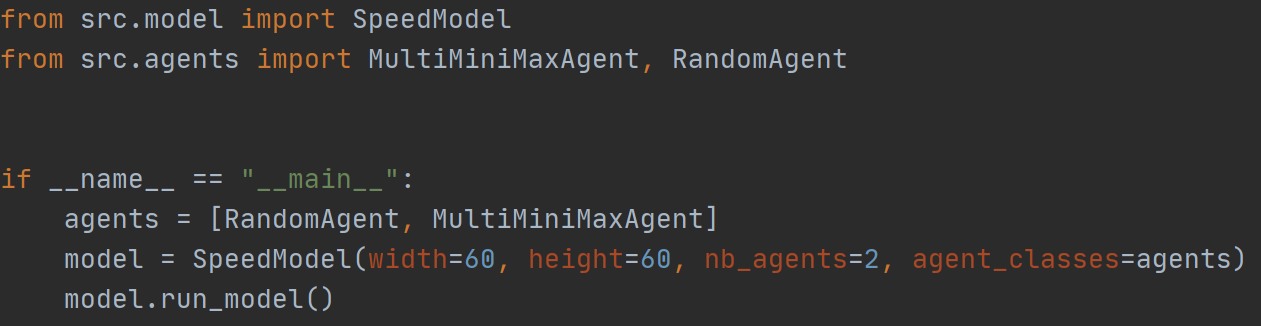
\includegraphics[width=0.9\textwidth]{img/model_code.PNG}
    \caption{Code-Beispiel zur Erstellung und Ausführung des Modells}
	\label{fig:model_code}
\end{figure}


\section{Software-Testing}
\label{sec:testing}

Das Schreiben von Software-Tests war für uns aus zwei Gründen besonders wichtig. Zum einen mussten wir sicher gehen können, dass unser Modell mit dem originalen Spiel übereinstimmt. Zum anderen war es wichtig, dass wir Erweiterungen und Optimierungen an den algorithmischen Ansätzen leicht validieren können. Die Tests sind - wie bei \textit{Unit Tests} in Python standardmäßig vorgesehen - in Software-Paketen namens \textit{tests}, auf gleicher Ebene wie das zu testende Modul, eingebettet.

Beim Testen des Modells kommt uns erneut die Black-Box-Eigenschaft zugute. Wir verwenden JSON-Dateien von gespeicherten Original-Spielen und gleichen in den Tests die Spielzustände zu jedem Zeitschritt mit denen unseres Modells ab. Dabei laden wir zuerst den initialen Spielzustand eines gespeicherten Spiels in das Modell, extrahieren dann die Aktionen der Spieler/Agenten zu den jeweiligen Zeitschritten und simulieren diese Aktionen dann auf unserem Modell. Wenn das Modell alle 58 gespeicherten Spiele korrekt simuliert, ist der Modell-Test bestanden. Auf diese Weise erhalten wir deutlich umfangreichere Tests, als durch manuelles Erstellen von Test-Spielzuständen möglich wäre.

Die implementierten Agenten und deren Algorithmen (Multi-Minimax, Voronoi, etc), werden mit Unit-Tests abgedeckt. Dabei testen wir, insbesondere ob die Agenten bei ausreichender Suchtiefe in verschiedenen Spielsituationen den besten Zug finden. Zu allen übrigen \textit{Core}-Softwaremodulen (wie z.B. \textit{utils}) haben wir ebenfalls Unit Tests geschrieben. Wie in Abbildung \ref{fig:coverage} zu sehen erreichen wir insgesamt eine Testabdeckung von 84\% für das \textit{Core}-Softwaremodul.

\begin{figure}[ht]
    \centering
    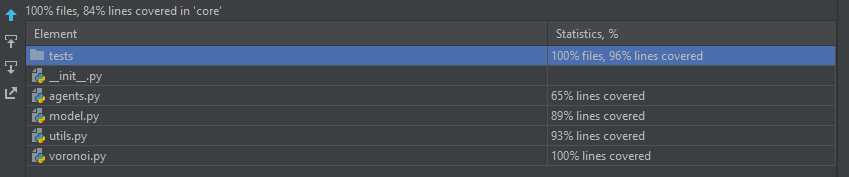
\includegraphics[width=0.9\textwidth]{img/coverage.PNG}
    \caption{Testabdeckung für das \textit{Core}-Softwaremodul}
	\label{fig:coverage}
\end{figure}